
\documentclass[11pt]{article}
\usepackage[margin=1in]{geometry}
\usepackage{amsmath,amssymb}
\usepackage{graphicx}
\usepackage{hyperref}
\usepackage{enumitem}
\usepackage{array}
\usepackage{fancyhdr}
\DeclareGraphicsExtensions{.png,.pdf}

\pagestyle{fancy}
\fancyhf{}
\fancyfoot[L]{\footnotesize Christian (Cruz) deWilde \& ChatGPT 5 (Thinking \& Pro) • ORCID: 0009-0008-5123-3556}
\fancyfoot[C]{\footnotesize OmniScale Gravity v3.7 (pandoc edition)}
\fancyfoot[R]{\footnotesize DOI: 10.5281/zenodo.16787984 • \thepage}
\setlength{\parindent}{0pt}
\setlength{\parskip}{0.65em}
\hypersetup{colorlinks=true,linkcolor=blue,urlcolor=blue,citecolor=blue}

\title{OmniScale Gravity (Expansion-as-Gravity) — Conservative Weak-Field Framework via $\chi$ (v3.7)}
\author{Christian (Cruz) deWilde\thanks{Independent Researcher (personal capacity). Employed by NVIDIA; work performed entirely on personal time and equipment.} \and ChatGPT 5 (Thinking \& Pro)}
\date{2025-08-13}

\begin{document}
\maketitle

\section*{Executive summary}
We package the tested, weak-field part of General Relativity (GR) in a simple scalar–metric language. A scalar field $\chi$ encodes \emph{differential expansion}: where $\chi$ changes across space, objects drift as if pulled by gravity. We keep the standard weak-field metric for optics and clocks, so classic tests (light bending, Shapiro delay, redshift, Mercury) are reproduced exactly (PPN $\gamma=1$). We adopt a conservative gravitational-wave sector (speed $c$, two tensor polarizations, no extra dipole channel). For cosmology, we introduce one small, dimensionless coupling $\alpha$ that links line-of-sight gradients to local $H_0$ estimates in a gauge-safe way. This produces falsifiable predictions (environment-dependent $H_0$, bulk flows aligned with $\nabla\chi$) under Solar-System and GW constraints.

\section*{Core equations with plain-English descriptions}
\textbf{E1 (prior, Poisson).} $\nabla^{2}\Phi = 4\pi G \rho$.
\emph{Meaning:} mass density $\rho$ sources the Newtonian potential $\Phi$.

\textbf{E2 (foundational identification; NEW).} $\boxed{\Phi = c^{2}\chi}$.
\emph{Meaning:} we posit that the gravitational potential is the expansion potential in units of $c^2$; this anchors the metric and keeps tested weak-field optics intact while making the expansion picture predictive.

\textbf{E3 (prior, motion).} $\ddot{\mathbf x} = -\nabla\Phi$.
\emph{Meaning:} objects accelerate down potential gradients.

\textbf{E4 (prior, gravitomagnetism).} $g_{0i} = -4 V_i / c^{3}$ with $V_i(\mathbf x)=G \int \rho(\mathbf x')\, v_i(\mathbf x')/\|\mathbf x-\mathbf x'\|\, d^{3}x'$.
\emph{Meaning:} moving matter drags inertial frames (Lense–Thirring).

\textbf{E5 (safe GW sector).} $(\partial_{t}^{2}-\nabla^{2})\,h_{ij}^{\mathrm{TT}}=0$, $v_{\mathrm{gw}}=c$, polarizations $+$ and $\times$.
\emph{Meaning:} we keep GR’s wave speed and polarizations; no kinetic mixing with $\chi$.

\section*{What is $H_0$? What is $\chi$? (8th-grade level)}
$H_0$ is the present-day Hubble constant (per second). It tells how fast distant galaxies recede on average. The scalar $\chi$ is a simple picture of expansion: if $\chi$ is steeper in one direction, motion drifts that way—like leaves moving toward the faster part of a river. In formulas we use the linear map $\Phi=c^{2}\chi$ so that standard tests follow directly; for storytelling in the infographic we sometimes write $\Phi_{\mathrm{eff}}=\frac{1}{2} c^{2}\|\nabla\chi\|^{2}$ to emphasize “big gradient → deep potential.”

\subsection*{What is PPN (one line)?}
PPN stands for ``Parametrized Post-Newtonian''—a bookkeeping system for small corrections to Newtonian gravity. The parameter $\gamma$ controls how space is curved by mass; GR predicts $\gamma=1$. Keeping $\gamma=1$ ensures that light bending and Shapiro delay come out exactly as in GR.

\section*{Parameter $\alpha$: gate checks and plan}
We link structure to local $H_0$ with one fitted parameter $\alpha$ through a gauge-safe LOS functional of $\nabla\Phi$. Gates: (i) Solar System optics (Cassini $|\gamma-1|$), (ii) GW speed/polarizations and pulsar dipole suppression, (iii) bulk-flow and ISW/CMB consistency. Plan: fit $\alpha$ with per-window histograms from real survey windows, while enforcing caps implied by these gates. We then cross-check against peculiar-velocity catalogs and $H_0$ anisotropy maps.

\section*{Predictions and falsifiers (front-page contract)}
Environment-dependent $H_0$ (voids higher, clusters lower), bulk flows aligned with $\nabla\chi$, lensing/time-delay consistency with GR optics, tiny lab effects in clocks/interferometers, and no Solar-System/GW violations. Failure modes: no $H_0$–environment correlation at the percent level, flows requiring an $\alpha$ that breaks Solar-System bounds, or lensing that demands $\gamma\neq1$.

\section*{Related work and novelty (brief bullets)}
Verlinde’s emergent gravity and McCutcheon’s expansion intuition share motifs but lack a standard PPN/GW sector; our novelty is an explicit $\chi\!\to\!\Phi$ identification that \emph{keeps} GR’s weak-field optics ($\gamma=1$) and a conservative wave sector, while yielding crisp, survey-scale predictions.

\section*{Scope note (conservative closure)}
We keep only the parts needed to reproduce tested weak-field physics and to state falsifiable survey predictions. Cosmological backreaction and a full $\chi$ field theory are left for future work; none of our near-term tests require them.

\section*{Implementation and pipeline}
We follow a simple run plan: per-window histograms of $\Delta H/H_0$ (median and 16–84 percentiles) from mixed void+cluster environments, with a single $\alpha$ and a Solar-System cap. Outputs include a \texttt{summary.json} with best-fit $\alpha$ and uncertainties.

\section*{Figures (with plain-English captions)}
\begin{figure}[h]\centering
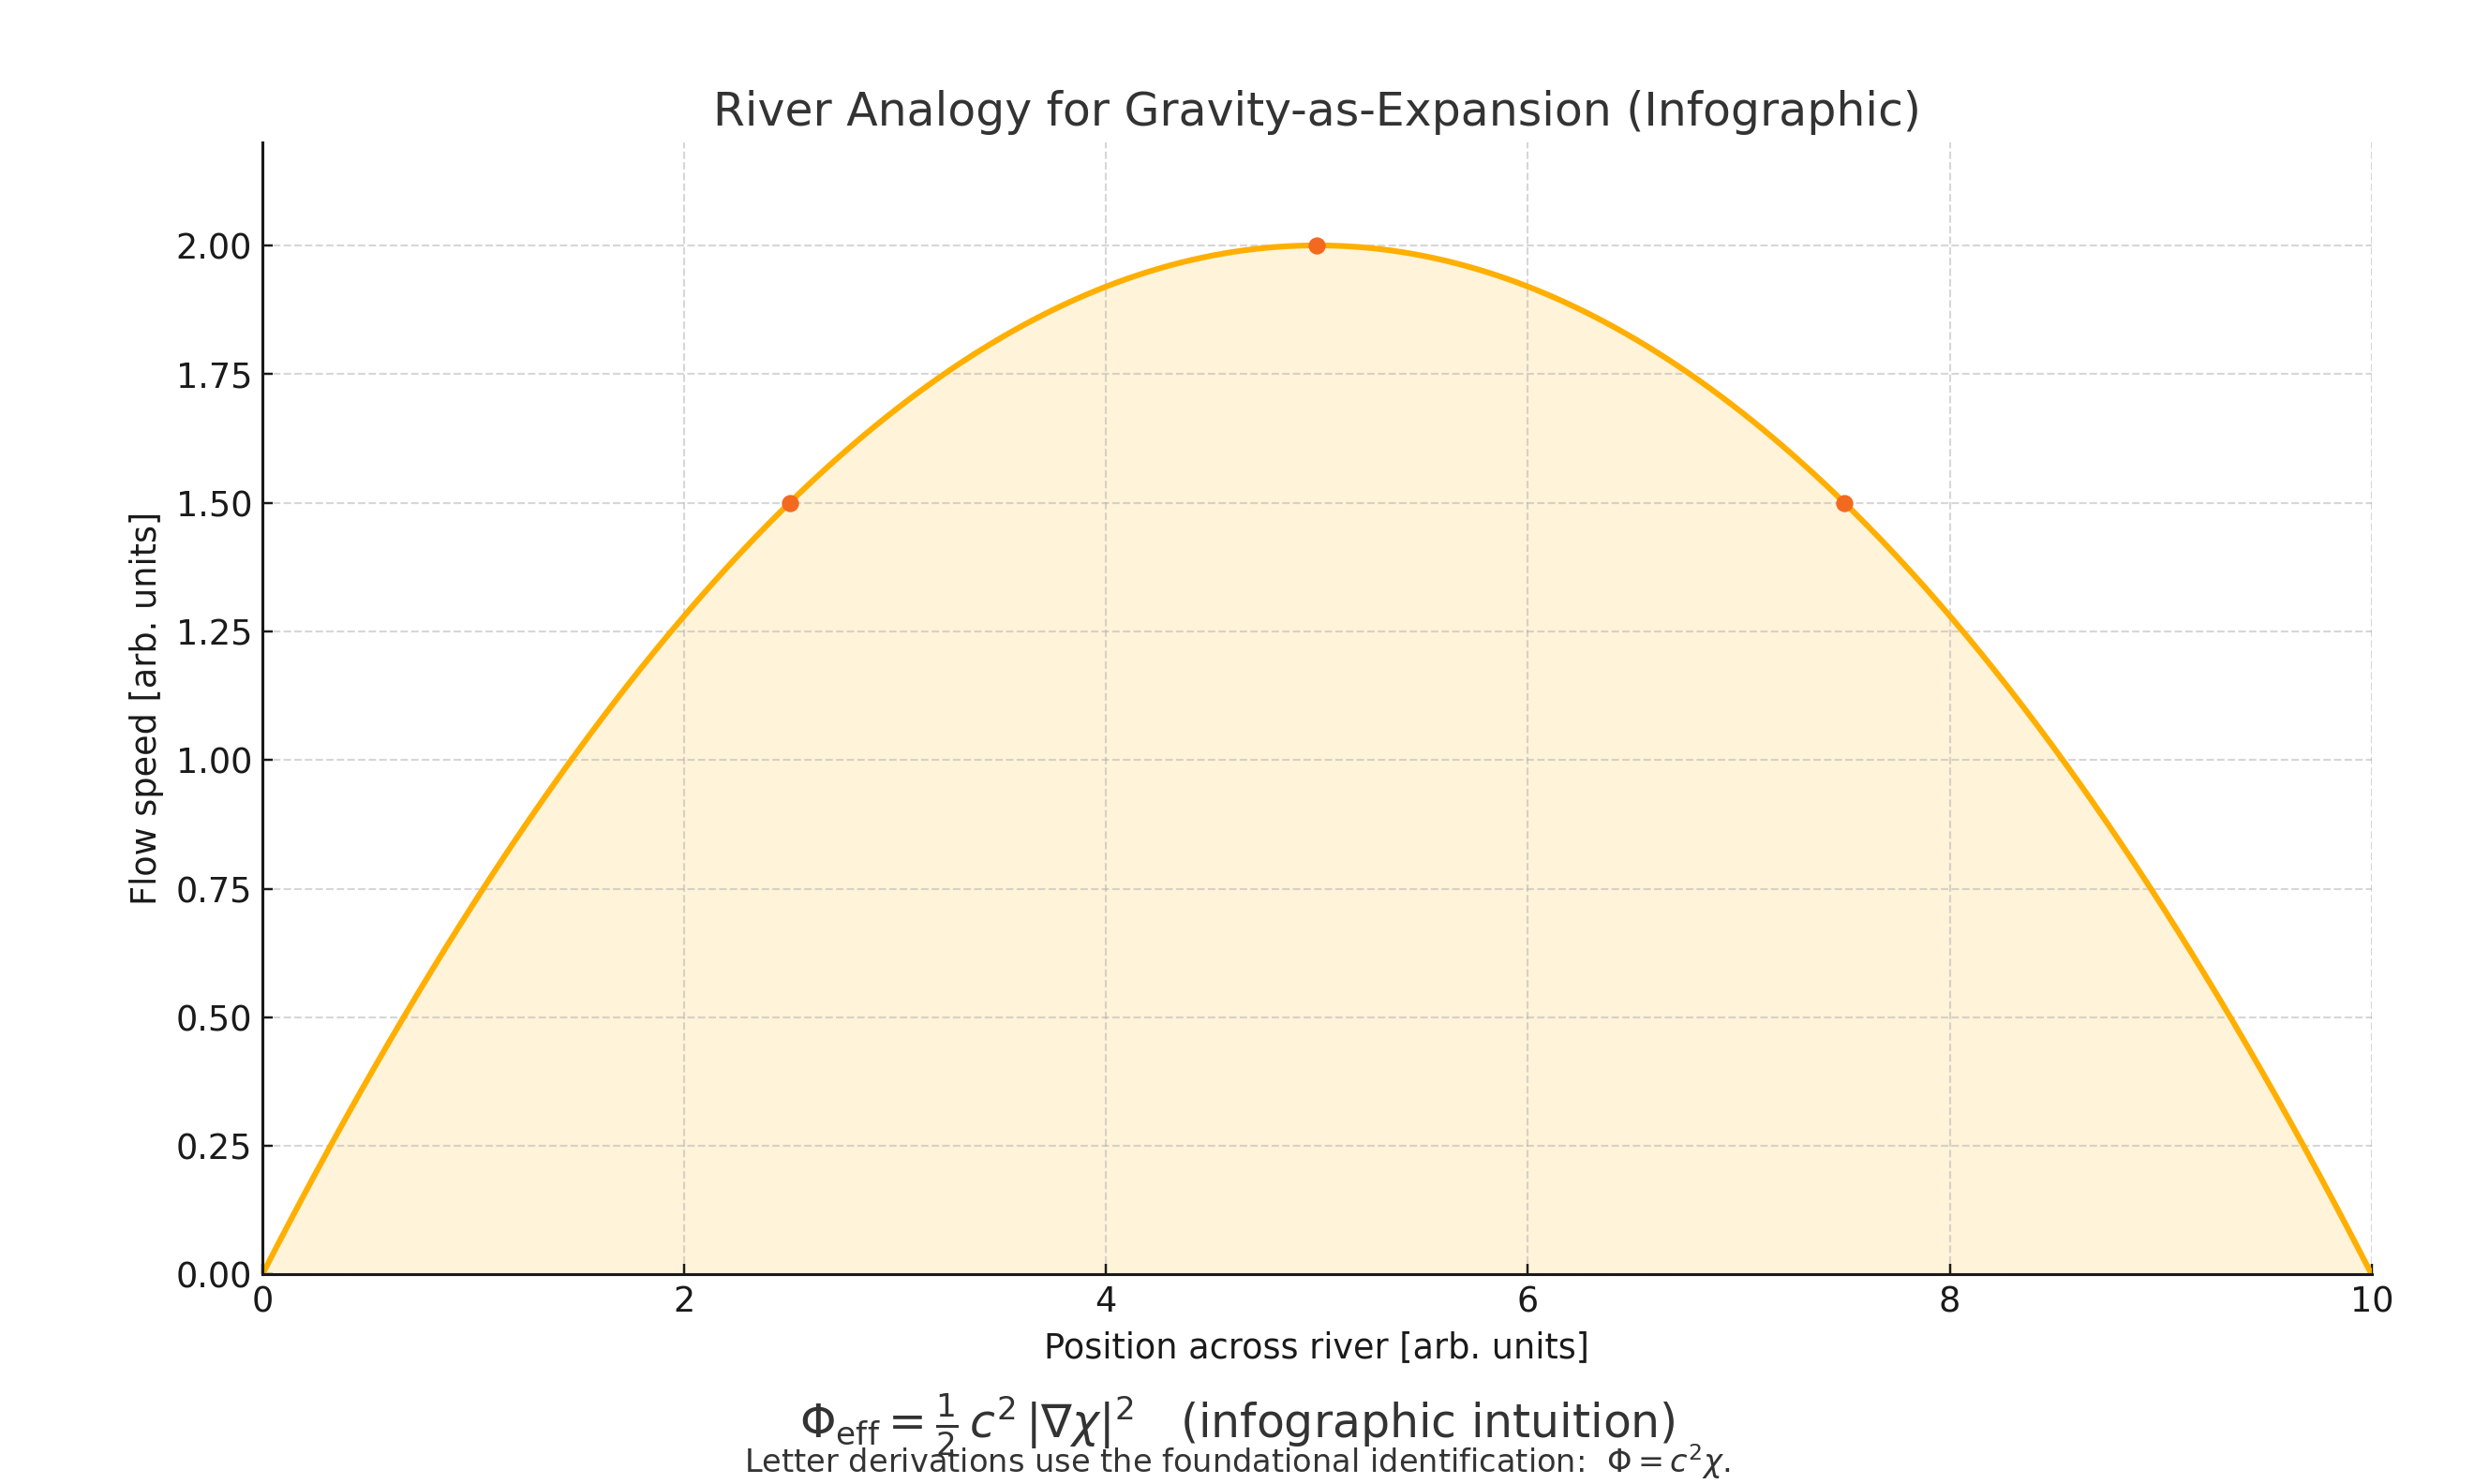
\includegraphics[width=0.92\linewidth]{expansion_gravity_infographic_v3_7.png}
\caption{\textbf{Infographic (river analogy).} Flow is faster in the middle and slower at the edges, so “leaves” drift sideways—like motion toward deeper gravitational regions. Equation shown is pedagogical ($\Phi_{\mathrm{eff}}=\frac{1}{2} c^{2}\|\nabla\chi\|^{2}$); derivations use $\Phi=c^{2}\chi$.}
\end{figure}

\begin{figure}[h]\centering
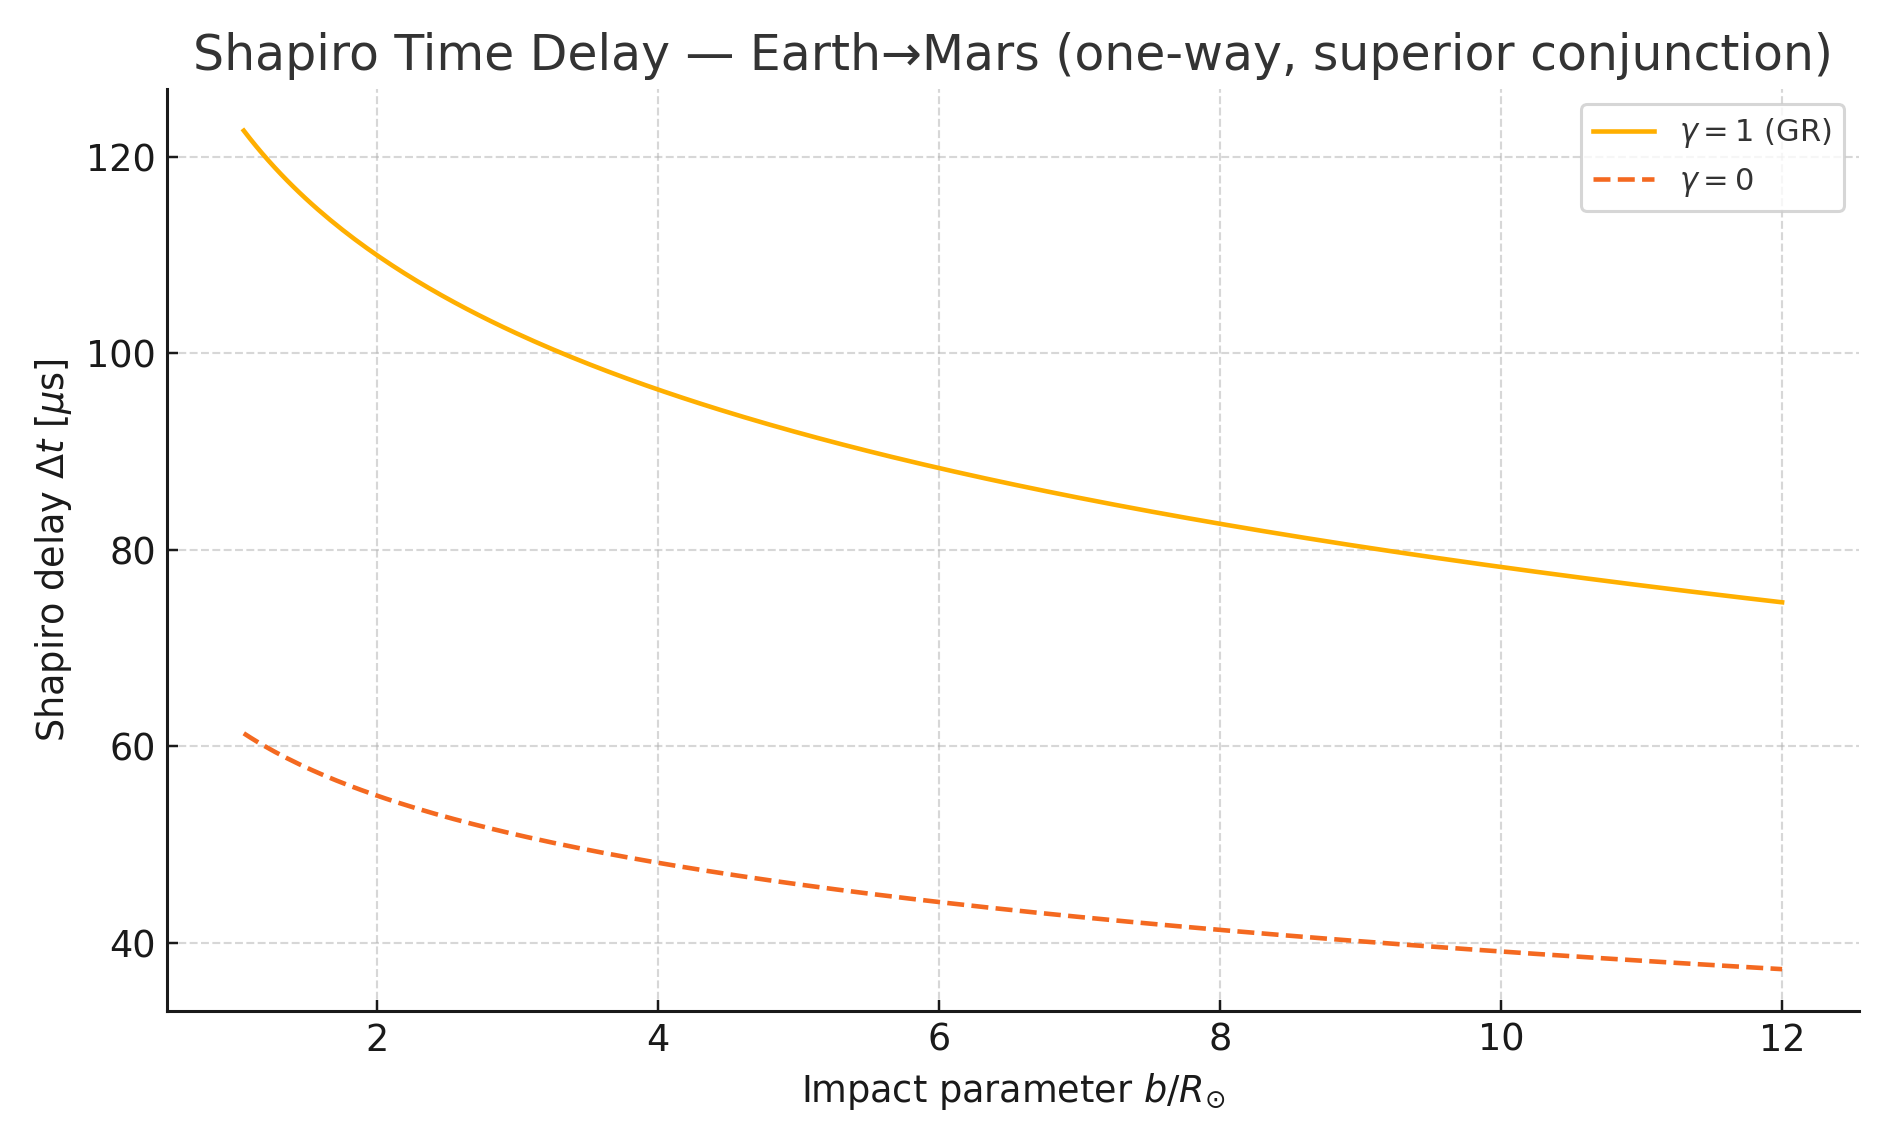
\includegraphics[width=0.82\linewidth]{shapiro_curves.png}
\caption{\textbf{Shapiro time delay (Earth–Mars, one-way).} Signals that pass near the Sun take slightly longer to arrive. The curve labeled $\gamma=1$ (GR) is the prediction we recover; a $\gamma=0$ reference is shown for comparison. The vertical axis is in microseconds; the horizontal axis is impact parameter in solar radii.}
\end{figure}

\section*{“Where does it come from?” (action, in plain English)}
Start from the standard Newtonian field action for $\Phi$ so that varying it gives Poisson’s equation. Substitute $\Phi=c^{2}\chi$. The resulting action for $\chi$ carries the same physics with fixed coefficients; no hand tuning is needed. This is why the metric built from $\Phi$ reproduces redshift, bending, Shapiro, and Mercury in the usual way.

\section*{Order-of-magnitude viability notes}
With a conservative kernel and small $\alpha$, the effect on $H_0$ is tiny, which is acceptable at this stage. To reach percent-level anisotropy, either the kernel or $\alpha$ must be calibrated against real selection functions and checked against bulk-flow/ISW caps—part of our plan.

\section*{Plain-English equation walkthrough (NEW vs PRIOR, why it matters)}
E1 and E3 are standard Newtonian/GR ingredients. E2 is our foundational identification that lets us speak directly in terms of an expansion map $\chi$ while preserving all tested predictions. The LOS equation connects this picture to cosmology via a single $\alpha$; choosing a gauge-safe kernel keeps units, signs, and interpretation straight.

\section*{Glossary of terms (what, and why it matters)}
$H_0$ — the present Hubble constant; baseline expansion rate.\\
$\chi$ — scalar expansion map; in formulas we use $\Phi=c^{2}\chi$.\\
$\Phi$ — potential used in the weak-field metric and motion; determines clocks, light paths, and orbits.\\
$\alpha$ — dimensionless coupling linking LOS structure to fractional $H_0$ shifts.\\
$W(s)$ — survey window (how many sources you have at distance $s$).\\
PPN — Parametrized Post-Newtonian; $\gamma=1$ means light responds to $\Phi$ exactly as in GR.\\
NFW cluster — Navarro–Frenk–White halo profile for clusters; describes how density falls with radius.\\
Eikonal — a ray-optics approximation; gradients of a “phase” guide rays. We use it only for intuition in the infographic.\\
H$_0$ bias distribution — a histogram showing how local $H_0$ estimates shift across many lines of sight.\\
Shapiro delay — extra time a signal takes when passing through a gravitational potential.\\
Mercury’s precession — the rotation of Mercury’s orbit ellipse, explained at 1PN order.

\section*{Summary: tests to pass and current status}
\begin{center}
\begin{tabular}{|p{0.26\linewidth}|p{0.33\linewidth}|p{0.18\linewidth}|p{0.18\linewidth}|}
\hline
\textbf{Test} & \textbf{What the theory says} & \textbf{Status now} & \textbf{Data gate}\\\hline
Light bending, Shapiro & Use GR weak-field metric with $\Phi$; PPN $\gamma=1$ & Matches by construction & Cassini-like bounds \\\hline
Redshift, Mercury & Standard 1PN formulae with $\Phi$ & Matches & Classic solar-system tests \\\hline
Frame dragging (LT) & Keep $g_{0i}=-4V_i/c^3$ & Target: match within errors & GP-B/LAGEOS \\\hline
GW sector & $v_{\mathrm{gw}}=c$, $+$ and $\times$ only; no mixing & Matches by assumption & LIGO/Virgo/KAGRA \\\hline
Binary pulsars & Quadrupole loss; scalar dipole $\approx 0$ & Matches if dipole $\ll 10^{-3}$ & Pulsar timing \\\hline
Local $H_0$ vs environment & $\Delta H/H_0 = \alpha \,\mathcal{I}[\nabla\Phi;W]$ & To be fitted & SN/standard-candle maps \\\hline
Bulk flows & Align with $\nabla\chi$; amplitude set by $\alpha$ & To be fitted & Cosmicflows/2M++ \\\hline
ISW / CMB lensing & Consistent late-time ISW for allowed $\alpha$ & To be checked & CMB–LSS x-correlations \\\hline
\end{tabular}
\end{center}

\section*{Acknowledgements}
We thank early readers and colleagues; maintainers of open-source tools; and the ephemeris, precision clock, gravitational-wave, and large-scale-structure communities whose public results constrain our safe-regime choices. We thank OpenAI for the wizardry behind ChatGPT. We are grateful to \textbf{Dr.\ Francisco Jose Ayala}, \textbf{Robert Ryan}, \textbf{Dr.\ Joon Yun}, and \textbf{Mariano Mu\~noz} for inspiring conversations, and we thank the human author's family for their support. Any errors remain our own.

\end{document}
